\documentclass{article}

\usepackage{amsmath, amsthm, bm, physics, enumerate, siunitx, dirtytalk, tikz}
\usepackage{hyperref}
\usetikzlibrary{calc, patterns}

\newtheorem{theorem}{Theorem}
% \newtheorem{lemma}{Lemma}

% \providecommand{\levicivita}[3]{%
%   \ensuremath{\varepsilon_{{#1}{#2}{#3}}}
% }


% ------------------------------------------------------------------------------
\title{Derivation of momentum conservation law\\
\large \textit{based on the lecture of prof.\ Andrzej Styczek}}
\author{Wojciech Sadowski}

\begin{document}
\maketitle

\section{Basics}

\paragraph{What is a fluid?}
We will consider a fluid as a continuous substance. That is, the fluid fills
fully available space. Therefore, \emph{we are neglecting the discrete nature
of matter.} We can do that, since the amount of fluid molecules in small volume 
of matter is gargantuan (remember the Avogadro number \(N_a\approx\SI{6.023e26}{kmol^{-1}}\)).

It is painfully difficult to describe the motion of each and every molecule 
constituting the fluid. Apart from the obvious problem of integrating all of 
the trajectories we also encounter a problem of determining an accurate initial
conditions for every molecule. In such systems, a small error in determining 
these starting parameters will unfortunately lead to considerable inaccuracies
further down the line.

Hence, we neglect the discrete nature of matter. The medium, i.e.\ fluid, consists 
of continuous set of ideal particles\footnote{%
A point that might have mass or charge or some other 
property. From Wikipedia: \say{an idealization of particles 
[...]. Its defining feature is that it lacks spatial extension; being dimensionless,
it does not take up space.}}.
So the movement of the medium is 
\emph{de facto} the movement of the points, and such description can be 
used for solids (a continuous medium retaining some shape or natural configuration),
fluids and \say{things} in between. Fluids do not have this natural, reference 
configuration: the relative positions of the points can be arbitrary and changing.
Sometimes we might assume that volume of fluid has to be conserved (or that the 
density is constant) but that is, of coarse, a simplification. A useful and 
accurate one in situations of non-varying thermodynamic state of the medium.

If this \say{reference shape} does not exist, than the deformation (or strain) of the fluid
can be completely arbitrary. \emph{Water spilled on the floor will deform greatly,
covering the area and seeping into the cracks, potentially making you call the 
handyman to fix the broken flooring.} So what creates the internal forces inside 
the fluid? One obvious answer is the change of volume, but what else?

We will consider fluids in which the forces depends on the rate of deformation. 
These forces clearly will \say{want} to stop, or counteract, the deformation 
occurring in the fluid. As we have already discussed, the deformation itself 
does not seem to be important.

However, it is important to indicate, that this is only a simplified model, 
not existing in nature. In the same way as each fluid is really compressible,
this assumption is a useful lie. For  
the most general fluid we could write
\[
  f(t, \bm{\tau}, \dot{\bm{\tau}}, \bm{D}, \dot{\bm{D}}, \dots) = 0,
\]
and call it \emph{constitutive equation}, i.e.\ a relation defining our material.
It describes connection between the time \(t\), stresses \(\bm{\tau}\), deformation \(\bm{D}\),
the rates of those things (indicated by the same letters with a dot accent) 
and potentially other parameters.

As you can see, it can be bad. The parameters in the above relations could
depend on each other or they could depend on each other non-locally (i.e.\ point
\(a\) depends on the state in point \(b\)). Or even worse, they might be influenced
by the history of the those parameters. Fortunately, for most of classical use 
cases we can confine ourselves to much simpler relations.

We will say:
\begin{enumerate}[(i)]
  \item only \(\bm{\tau}\) and \(\dot{\bm{D}}\) are important;
  \item the relation between them is defined in the same place and time;
  \item we should be able two solve for \(\bm{\tau}\), that is write
    \[
      \bm{\tau} = g\qty(\dot{\bm{D}}).
    \]
\end{enumerate}

\paragraph{What are stresses?}
We know what a \emph{force} is. Intuitively,
when thinking about fluids or materials, the stress is a force acting on 
a surface. We also know that we can add forces, so we can safely assume that
the sum of forces acting on parts of the surface have to add up to the force 
acting on the whole surface. Let's define force differential \(\dd{\vb{F}}\) acting 
on a small part of the surface \(\dd S\), in a following way
\[
  \dd \vb{F} = \vb{f}\dd{S},
\]
so that \(\vb{f}\) becomes a force per unit surface, so surface force density.

Let us consider a Cartesian coordinate system \((O, x_1, x_2, x_3)\) and 
a small tetrahedron with walls \(\dd S_1\), \(\dd S_2\), \(\dd S_3\) and 
closed by the wall \(\dd S\) (see \autoref{fig::force_tetrahedron}). There 
can be infinite amount of such tetrahedrons, however the numbered walls 
\(\dd S_i\) are always laying on the same planes, perpendicular to the 
axis of the system. On the other hand, wall \(\dd S\) changes its position
along with the plane its laying on and the surface area. 

\begin{figure}[bh!]
  \centering
  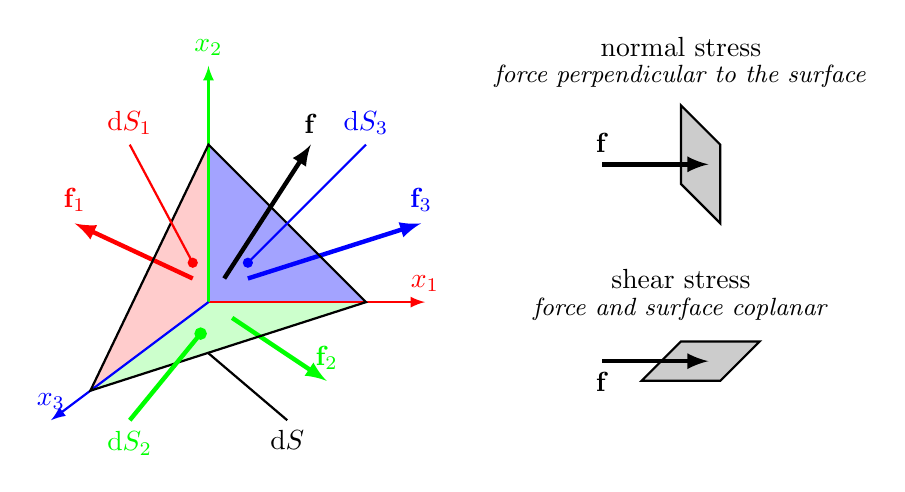
\begin{tikzpicture} 
    \fill [red, fill opacity = 0.2] (0cm, 0cm) -- (-2cm * 0.75, -1.5cm * 0.75) -- (0cm, 2cm) -- cycle;
    \fill [green, fill opacity = 0.2] (0cm, 0cm) -- (-2cm * 0.75, -1.5cm * 0.75) -- (2cm, 0cm) -- cycle;
    \fill [blue, fill opacity = 0.2] (0cm, 0cm) -- (2cm, 0cm) -- (0cm, 2cm) -- cycle;
    \fill [blue, fill opacity = 0.2] (0cm, 0cm) -- (2cm, 0cm) -- (0cm, 2cm) -- cycle;
 
    \draw [red, -latex, ultra thick] 
    (-0.2cm, 0.3cm) -- (-1.7cm, 1cm) node [above] {$\vb{f}_1$}; 
    \draw [blue, -latex, ultra thick] 
    (0.5cm, 0.3cm) -- (2.7cm, 1cm) node [above] {$\vb{f}_3$}; 
    \draw [green, -latex, ultra thick] 
    (0.3cm, -0.2cm) -- (1.5cm, -1cm) node [above] {$\vb{f}_2$}; 

    \draw [-latex, thick, red] (0cm, 0cm) -- (2.75cm, 0cm) node [above] {$x_1$};
    \draw [-latex, thick, green] (0cm, 0cm) -- (0cm, 3cm) node [above] {$x_2$};
    \draw [-latex, thick, blue] (0cm, 0cm) -- (-2cm, -1.5cm) node [above] {$x_3$};
    \draw [thick] (-2cm * 0.75, -1.5cm * 0.75)  -- (2cm, 0cm) -- (0cm, 2cm) -- cycle;
    % \fill [pattern=north west lines, pattern color=black] (-2cm * 0.75, -1.5cm * 0.75)  -- (2cm, 0cm) -- (0cm, 2cm) -- cycle;
    
    \draw [blue, thick] (0.5cm, 0.5cm) -- (2cm, 2cm)
      node [pos=1, above] {$\dd S_3$}  
      node [draw=blue, circle, fill=blue, inner sep=1pt, pos=0]  {}; 
    \draw [red, thick] (-0.2cm, 0.5cm) -- (-1cm, 2cm)
      node [pos=1, above] {$\dd S_1$}  
      node [draw=red, circle, fill=red, inner sep=1pt, pos=0]  {}; 
    \draw [green, ultra thick] (-0.1cm, -0.4cm) -- (-1cm, -1.5cm)
      node [pos=1, below] {$\dd S_2$}  
      node [draw=green, circle, fill=green, inner sep=1pt, pos=0]  {}; 
    \draw [black, thick] (0cm, -0.65cm) -- (1cm, -1.5cm)
      node [pos=1, below] {$\dd S$};

    \draw [ultra thick, -latex] (0.2cm, 0.3cm) -- (1.3cm, 2cm) 
      node [above] {$\vb{f}$};

    % \node at (4cm, 3cm) [anchor = north west] {%
    %   \parbox{4cm}{%
    %   Equilibrium condition:\\
    %   \(\vb{f}_i \dd S_i+ \vb{f}\dd S =\vb{0}\)
    %   }};
    \begin{scope}[xshift=1cm]
    \draw [fill, color = black, fill opacity=0.2, thick] 
      (5cm, 2.5cm) -- (5.5cm, 2cm) 
      -- (5.5cm, 1cm) -- (5cm, 1.5cm) -- cycle ;
    \node at (5cm, 3cm) [above] {normal stress};
    \node at (5cm, 2.60cm) [above] 
    {\small \textit{force perpendicular to the surface}};
  
    \draw [-latex, ultra thick] (4cm, 1.75cm) -- (5.35cm, 1.75cm)
      node [above, pos=0] {$\vb{f}$};

    \node at (5cm, 0.05cm) [above] {shear stress};
    \node at (5cm, -0.35cm) [above] 
    {\small \textit{force and surface coplanar}};
    \draw [fill, color = black, fill opacity=0.2, thick]
      (5cm, -0.5cm) -- (6cm, -0.5cm) -- (5.5cm, -1cm) 
      -- (4.5cm, -1cm) -- cycle;
    \draw [-latex, ultra thick] (4cm, -0.75cm) -- (5.35cm, -0.75cm)
      node [below, pos=0] {$\vb{f}$};
    \end{scope}
  \end{tikzpicture}
  \caption{Elementary tetrahedron}
  \label{fig::force_tetrahedron}
\end{figure}

If this volume is in equilibrium, than the forces acting on the walls, 
\(\vb{f}_1\), \(\vb{f}_2\), \(\vb{f}_3\) and \(\vb{f}\) respectively,
add up to \(\vb{0}\)
\begin{equation}\label{eq::equilibrium}
  \vb{f}_1 \dd{S_1} 
  + \vb{f}_2 \dd{S_2} 
  + \vb{f}_3 \dd{S_3} 
  + \vb{f} \dd{S} = \vb{f}_i \dd{S_i} + \vb{f} \dd{S} = \vb{0}.
\end{equation}
Let us divide the equation by \(\dd{S}\)
\[
  \vb{f}_i \dfrac{\dd{S_i}}{\dd{S}} + \vb{f} = \vb{0}.
\]
We do that because we notice that the fraction \(\dd{S} / \dd{S_i}\) is
equal to the cosine of the angle between the normal of \(\dd{S}\) and 
the \(i\)-th axis of the coordinate system (believe me, or prove it 
if you don't). We can also say that \(\cos(\bm{n}, x_i) = n_i\) and we will
use that later. 

In \autoref{eq::equilibrium} we didn't assume anything about the directions
of the forces, however, if the tetrahedron is in equilibrium, than the sum of 
\(\vb{f}_i\) has to be opposite to \(\vb{f}\). Hence, we can flip it noting
that if we change direction, the sign changes as well, i.e.\ 
\(\vb{f}(\vb{n}) = -\vb{f}(-\vb{n})\). 
After substituting our \say{revolutionary} findings about the 
\(\dd{S} / \dd{S_i}\) ratio equal to the cosine as well, we are left with the following relation
\[
  \vb{f} = \vb{f}_i \dfrac{\dd{S_i}}{\dd{S}} 
  = \vb{f}_i\cos(\bm{n}, x_i) 
  = \vb{f}_i n_i  
\]

Now, considering that each force has three components, which for example for 
\(\vb{f}_1\) we will denote as \(f_{11}\), \(f_{12}\) and \(f_{13}\), we can 
also write the equation for \(k\)-th component of \(\vb{f}\)
\[
  f_k = n_1 f_{1k} + n_2 f_{2k} +n_3 f_{3k} = n_\alpha f_{\alpha k}.
\]
So, we actually have arrived at something! We have \emph{nine} numbers giving
together the components of \(f_{\alpha k}\), which describe the forces acting 
on the surface closing our small tetrahedron. Furthermore, if you shrink the 
tetrahedron to a point (we already used differentials of surfaces), what we 
wrote above still holds! This means that, the force density acting on a surface 
in the fluid depends on those nine numbers and the orientation of the surface.

We will call those numbers stresses. Make a though experiment: imagine a force 
acting in a chosen direction, and a surface perpendicular to this force. This 
is aligned with the classical definition of pressure, right? Now, rotate this 
surface, so that the force vector lies on the surface. Force acting along the 
surface can be understood as shear. That's how scissors work! Now, rotate the 
surface keeping the normal as an axis. The force is now \say{shearing} the 
surface in a different direction, so for one force vector we can have one normal 
(perpendicular to the surface)
stress and we observed two shear stresses. With that (hopefully) intuitive 
explanation we can say that among the nine numbers, we will have \emph{three}
normal stress components and \emph{six} components related to shear stress.

The only problem is the fact that our notation is cumbersome; we have two \(f\)
symbols. Let's set the magic nine numbers (they will get a name soon, I promise!) 
as \(\tau_{ij}\), giving us:
\[
  f_i = n_\alpha \tau_{\alpha i}
\]

\paragraph{Stress tensor}
Okay, so as I said, the nine-number-thingy needs a name. You saw the paragraph
title, you might already now what it is. That said, this is written in style of 
a lecture, so please make a dramatic pause in your brain before reading the end of the 
next sentence. We will call \(\tau_{ij}\) the \emph{stress tensor}. 

But what is a tensor, you might ask? The mathematical definition is convoluted and 
hard. Truthfully, even I, \emph{the oh-so-smart author}, am not fully equipped 
mathematically to answer this question fully and correctly. So we will cheat 
and describe a tensor with as much verbosity as is necessary for our use case.

Let's define some operations first and show them on the example of the stress 
tensor, which we will represent here as
\[
  \bm{\tau} = \tau_{ij}\hat{\vb{e}}_i \hat{\vb{e}}_j.
\]
We used the versors \(\hat{\vb{e}}_i\) defining our chosen coordinate system. 
They are multiplied in a weird way, its neither scalar nor vector product. This 
operation is also sometimes written with 
the \(\otimes\) symbol (\(\hat{\vb{e}}_i \otimes \hat{\vb{e}}_j\)) and 
is called tensor or outer product.

The scalar product \(\vb{n}\dotproduct\bm{\tau}\) can be written easily 
with index notation. We know that \(\vb{n} = n_k \hat{\vb{e}}_k\), so 
building on that we can write
\[
  \vb{n}\dotproduct\bm{\tau} 
  = n_k \hat{\vb{e}}_k \dotproduct \qty(\tau_{ij}\hat{\vb{e}}_i \hat{\vb{e}}_j)
  = n_k \tau_{ij} \hat{\vb{e}}_k \dotproduct \hat{\vb{e}}_i \hat{\vb{e}}_j 
  = n_k \tau_{ij} \qty(\hat{\vb{e}}_k \dotproduct \hat{\vb{e}}_i) \hat{\vb{e}}_j.
\]
We can think a little about the term \(\hat{\vb{e}}_k \dotproduct \hat{\vb{e}}_i\).
It is a dot product of two versors. It can be either equal to 1 if they are 
the same (\(k=i\)) or 0 if they are different. There is a term for that, called
\emph{Kronecker delta}, defined as
\[
  \delta_{ij} = \begin{cases}
0 &\text{if } i \neq j,   \\
1 &\text{if } i=j.   \end{cases}
\]
So we can write that our product is equal to 
\(n_k \tau_{ij}\delta_{ki} \hat{\vb{e}}_j \). It does not help us yet, but if 
we said that \(k\) has to be equal to \(i\), otherwise the terms in the sum 
will be 0, we might as well write \(i\) instead of \(k\)\footnote{If you are 
confused try it out on paper, write every term, eliminate the ones equal to 0
and collapse the term to the indexed expression.}, i.e.\
\[
  \vb{n}\dotproduct\bm{\tau} = n_i \tau_{ij} \hat{\vb{e}}_j = f_j \hat{\vb{e}}_j.
\]
In the above, we eliminated \(\delta_{ii}\) as it is always equal to 1. In fact,
\(\delta_{ij}\) is sometimes called an \say{index renamer} as it renames index 
\(j\) to \(i\) or \textit{vice versa}.

Okay, so what have we learned? The dot product of a tensor with a vector gives 
us a vector. Will multiplication from the left, which we performed above, be 
different from the one from the right, that is \(\bm{\tau}\dotproduct\vb{n}\)?
Yes\footnote{I am to lazy to write it down, but it might be a good training
for you.}. That said, it would be the same if \(\tau_{ij} = \tau_{ji}\).

So a lot of hints have been dropped. The tensor behaves a little bit like a 
matrix. In fact the matrix is often used to \emph{represent} a tensor in a 
chosen coordinate system, but the tensor itself, like a velocity vector, is 
independent from the chosen coordinate system\footnote{Turns out the velocity 
vector is also a tensor of rank 1. Stress tensor has rank 2; we used two versors, 
so called diad, to define it.}. This matrix can be multiplied with a vector to give 
another vector. If the matrix is symmetric, product from both sides will return vectors 
with the same components. Kronecker delta is also a tensor itself, represented by
a unit matrix \(\bm{I}\).

\paragraph{Strain-rate (deformation-rate) tensor}
It was mentioned, that we are interested in a tensor defining a rate of 
deformation, or what is usually called \emph{strain-rate tensor} in 
literature. We should derive it. Let's start with a series expansion of 
velocity field around coordinate \(\vb{r}\):
\[
  v_i(t, \vb{r} + \dd{\vb{x}}) = v_i(t, \vb{r}) + \pdv{v_i}{x_k}\dd{x_k}
  + \dots
\]
If \(\dd{x}\rightarrow\vb{0}\), we disregard the higher order terms and 
rewrite the above as 
\[
  v_i(t, \vb{r} + \dd{\vb{x}}) = v_i(t, \vb{r}) 
  + \frac{1}{2}\qty(\pdv{v_i}{x_k} + \pdv{v_k}{x_i})\dd{x_k}
  + \frac{1}{2}\qty(\pdv{v_i}{x_k} - \pdv{v_k}{x_i})\dd{x_k}.
\]
The first term on the right describes simple translation of the fluid parcel.
The third (similar to the expression for the curl of velocity field) defines
rotation. Both of these can be applied to the rigid, unchanging in shape, 
fluid parcel. We are left with the second one, describing the change of 
velocity due to \say{non-rigid} strain or deformation of the fluid volume. 
We can write this change of velocity mathematically as
\[
  \dd{v^\mathrm{strain}_k} 
  = \frac{1}{2}\qty(\pdv{v_i}{x_k} + \pdv{v_k}{x_i})\dd{x_k}
  = \dot{D}_{ik}\dd{x_k}
\]
The tensor \(\dot{\vb{D}}\) is the strain-rate tensor and very importantly 
it is \emph{symmetric}!

\section{Momentum equation I: General form}

\section{Fluid constitutive relations}

\section{Momentum equation II: Navier-Stokes}

% \begin{proof}
%   The triangle \(\dd{S}\) is span by the vectors \(\bm{\eta}_i\) laying 
%   along the axes of the system. Therefore, the area of \(\dd{S}\) is given
%   as
%   \[
%     \dd{S} = \frac{1}{2} \qty(\bm{\eta}_1 - \bm{\eta}_2)
%     \cross  \qty(\bm{\eta}_1 - \bm{\eta}_3),
%   \]
%   and similarity for \(\dd{S_1}\)
%   \[
%     \dd{S_i} = \frac{1}{2} \bm{\eta}_2 \cross  \bm{\eta}_3.
%   \]
%   So, the fraction of areas can be computed as
%   \[
%     \frac{\dd{S_1}}{\dd{S}} 
%     = \frac{%
%       |\bm{\eta}_2| |\bm{\eta}_3| \sin(\bm{\eta}_2, \bm{\eta}_3)}{%
%       \qty|\bm{\eta}_1 - \bm{\eta}_2|\qty|\bm{\eta}_1 - \bm{\eta}_3| 
%       \sin(\bm{\eta}_1 - \bm{\eta}_2, \bm{\eta}_1 - \bm{\eta}_3)  }.
%   \]
%   We can simplify, by noting that certain vectors lie along the axis of 
%   the system:
%   \[
%     \frac{\dd{S_1}}{\dd{S}} 
%     = \frac{%
%       \eta_2 \eta_3 }{%
%         \sqrt{\eta^2_1 + \eta_2^2} \sqrt{\eta^2_1 + \eta_3^2} 
%         \sin(\bm{\eta}_1 - \bm{\eta}_2, \bm{\eta}_1 - \bm{\eta}_3)  }
%       = \frac{1/\sin(\bm{\eta}_1 - \bm{\eta}_2, \bm{\eta}_1 - \bm{\eta}_3)
%       }{\sqrt{\dfrac{\eta_1^2}{\eta_2^2}+1}\sqrt{\dfrac{\eta_1^2}{\eta_3^2}+1}}.
%   \]
% \end{proof}




\end{document} 
